\documentclass[article]{jss}\usepackage[]{graphicx}\usepackage[]{xcolor}
% maxwidth is the original width if it is less than linewidth
% otherwise use linewidth (to make sure the graphics do not exceed the margin)
\makeatletter
\def\maxwidth{ %
  \ifdim\Gin@nat@width>\linewidth
    \linewidth
  \else
    \Gin@nat@width
  \fi
}
\makeatother

\usepackage{Sweave}



%% ----- Front matter (JSS template fields) ------------------------------------
\author{Mike Nguyen}
\Plainauthor{Mike Nguyen}

\title{\pkg{regsensitivity}: Sensitivity Analysis for Omitted Variable
       Bias in Linear Regression in \proglang{R}}
\Plaintitle{regsensitivity: Sensitivity Analysis for Omitted Variable Bias
            in Linear Regression in R}
\Shorttitle{\pkg{regsensitivity}: OVB Sensitivity in \proglang{R}}

\Abstract{
Sensitivity analysis for omitted variable bias has become a routine step in
applied regression work, and the methodological literature has produced a
sequence of increasingly general results. A recurring limitation of the
most widely used tools is that they assume the included control variables
are themselves exogenous, an assumption that is rarely defensible and whose
failure can reverse a robustness verdict. \citet{Diegert2026} derive sharp
identified sets for a regression coefficient that remain valid when the
controls are arbitrarily endogenous, indexed by three interpretable
sensitivity parameters. This paper introduces \pkg{regsensitivity}, an
\proglang{R} package implementing those results together with the related
analyses of \citet{Oster2019} and \citet{Masten2026}, under a single
formula-based interface. Beyond porting the methodology, the package
contributes bootstrap inference for the breakdown point, which
\citet{Diegert2026} explicitly leave to future work, and we report a
simulation study of its finite-sample coverage. We describe the underlying
identification theory, the regime dispatch that the three-parameter
problem requires, the package design and API, a replication of the
\citet{BFG2020} application that reproduces every value of
\citet{Diegert2026} Table 1 column (5) and Tables 3 and 4, two further
applications, and a comparison with \pkg{sensemakr} \citep{Cinelli2020}.
A suite of 26 paper-exact regression tests pins the replicated values to
within one unit in the last published digit.
}

\Keywords{omitted variable bias, sensitivity analysis, breakdown point,
          endogenous controls, identified set, \proglang{R},
          \pkg{regsensitivity}}
\Plainkeywords{omitted variable bias, sensitivity analysis, breakdown point,
               endogenous controls, identified set, R, regsensitivity}

\Address{
  Mike Nguyen\\
  ORCID: \url{https://orcid.org/0000-0002-3432-8595}\\
  URL: \url{https://github.com/mikenguyen13/regsensitivity}
}

%% ----- Style ----------------------------------------------------------------
\usepackage{amsmath,amssymb,amsthm,bm}
\usepackage{booktabs}
\usepackage{tikz}

\newcommand{\Rlang}{\proglang{R}}
\newcommand{\Stata}{\proglang{Stata}}
\newcommand{\blong}{\beta_{\mathrm{long}}}
\newcommand{\bmed}{\beta_{\mathrm{med}}}
\newcommand{\bshort}{\beta_{\mathrm{short}}}
\newcommand{\rxbar}{\ensuremath{\overline{r}_X}}
\newcommand{\rybar}{\ensuremath{\overline{r}_Y}}
\newcommand{\cbar}{\ensuremath{\overline{c}}}
\newcommand{\clow}{\ensuremath{\underline{c}}}
\newcommand{\Rsq}[1]{\ensuremath{R^2_{#1}}}
\newcommand{\Var}{\operatorname{var}}
\newcommand{\Cov}{\operatorname{cov}}

%% ----- knitr setup ----------------------------------------------------------


\IfFileExists{upquote.sty}{\usepackage{upquote}}{}
\begin{document}

%% ============================================================================
\section{Introduction}\label{sec:intro}
%% ============================================================================

A central concern in empirical research with observational data is that the
coefficient of interest in a linear regression may be biased because a
relevant covariate has been omitted. The applied literature has long sought
tools that quantify this concern: \emph{how much} omitted-variable bias
would there have to be in order to overturn the conclusion?
\citet{Altonji2005} introduced the heuristic of comparing the strength of
selection on observables to selection on unobservables;
\citet{Oster2019} formalized that heuristic and gave a specific
quantity~$\delta$ summarizing the relative strength; \citet{Cinelli2020}
recast the question in terms of partial $R^2$ between the unobservable and
the regressors; and \citet{Masten2026} identified an asymmetry in the Oster
framework that matters when one is interested in sign changes rather than
zero crossings. Related approaches include \citet{Imbens2003},
\citet{Hosman2010}, \citet{HsuSmall2013}, \citet{Krauth2016} and, in the
nonparametric setting, \citet{Rosenbaum2002}, \citet{Tan2006} and
\citet{Masten2018}.

Almost all of this work shares an assumption that is easy to overlook: the
included control variables are exogenous, in the sense of being uncorrelated
with the omitted variable. That assumption is rarely defensible. Controls
are typically chosen because they proxy for the same latent forces that the
omitted variable represents, so if the omitted variable is a geographic or
climatic factor and the controls are geographic and climatic variables, they
will be correlated almost by construction. \citet{Diegert2025} show
formally that residualization, the literature's most common device for
accommodating endogenous controls, can deliver incorrect robustness
conclusions; \citet{DeLuca2019}, \citet{Frolich2008} and
\citet{Hunermund2025} document further difficulties with control variables
in this setting.

\citet{Diegert2026}, hereafter DMP, respond by deriving sharp identified
sets for the coefficient of interest that remain valid when the controls
are \emph{arbitrarily} endogenous. Their analysis is indexed by three
interpretable sensitivity parameters, and it nests the exogenous-control
case as a special case, so the two can be compared within one framework.
It is this analysis, together with the closely related work of
\citet{Oster2019} and \citet{Masten2026}, that the \pkg{regsensitivity}
package implements.

These methods are heavily used---\citet{Oster2019} alone has been cited
more than five thousand times---but a complete \Rlang\ implementation has
not been available. Section~\ref{sec:landscape} surveys the existing
\Rlang\ and \Stata\ ecosystem in detail; in summary, the available
\Rlang\ packages implement either Oster's $\delta$ alone (\pkg{robomit},
\citealp{robomit}), the \citet{Cinelli2020} robustness value alone
(\pkg{sensemakr}, \citealp{sensemakr}), or related but distinct
diagnostics (\pkg{konfound}, \citealp{konfound}; \pkg{causalsens},
\citealp{causalsens}; \pkg{tipr}, \citealp{tipr}), and none of them allow
for endogenous controls or expose the breakdown frontier as a
programmable object.

\subsection{Contributions}

This paper introduces \pkg{regsensitivity} for \Rlang. The package
implements every closed-form regime of the DMP analysis, the nonconvex
regime requiring global optimization, the \citet{Oster2019} cubic-root
identified set, and the \citet{Masten2026} maximum-omitted-variable-bias
extension. Concretely, it offers:

\begin{itemize}
\item A \code{formula}-and-\code{data.frame} interface that fits naturally
into existing \Rlang\ workflows, with a control/calibration covariate
split expressed through a single \code{compare} argument.
\item Native \pkg{ggplot2} \citep{ggplot2} rendering of the identified set
and the breakdown frontier, with full theming and faceting support.
\item Percentile and cluster-robust bootstrap confidence intervals for the
breakdown point. DMP state that they ``expect the corresponding asymptotic
theory for estimation and inference on the bound functions to be
straightforward, but for brevity we do not develop it'' (Section 3.6).
The package therefore supplies the inferential step that the identification
paper leaves open, and Section~\ref{sec:case-sim} reports a simulation
study of its coverage.
\item A reproducibility test layer: 26 \pkg{testthat} assertions (across
six \code{test\_that} blocks) pin \citet{Diegert2026} Table 1 column (5)
and Tables 3 and 4 to within one unit in the paper's last printed digit, so
future numerical changes---a dependency update, a refactor---break loudly
rather than silently.
\end{itemize}

Section~\ref{sec:model} sets out the model and notation.
Section~\ref{sec:dmp} presents the DMP identification results and maps each
to the function that implements it. Section~\ref{sec:related} covers the
Oster and Masten--Poirier analyses and gives a crosswalk between the three
parameterizations. Section~\ref{sec:landscape} surveys existing software.
Section~\ref{sec:software} describes the package design.
Section~\ref{sec:api} is a tutorial introduction to the API.
Section~\ref{sec:replication} replicates the DMP application.
Sections~\ref{sec:case-school} and~\ref{sec:case-sim} apply the package to
a California schools regression and to a simulation study of bootstrap
coverage. Section~\ref{sec:compare} compares with \pkg{sensemakr}.
Section~\ref{sec:bench} reports benchmarks and
Section~\ref{sec:concl} concludes.

%% ============================================================================
\section{The model}\label{sec:model}
%% ============================================================================

Let $Y$ and $X$ be observed scalar variables, let $W_1$ be a vector of
observed covariates of dimension $d_1$, and let $W_2$ be an unobserved
vector. Write $W := (W_1, W_2)$. Throughout we assume the variance matrix
of $(Y, X, W_1, W_2)$ is finite and positive definite, which is what makes
the population linear regressions below well defined. The long regression
is
\begin{equation}
Y = \blong X + \gamma_1' W_1 + \gamma_2' W_2 + Y^{\perp X, W},
\label{eq:longreg}
\end{equation}
where $Y^{\perp X,W}$ denotes the linear projection residual plus
intercept, and is by construction uncorrelated with $(X, W)$. The target of
inference is $\blong$. The first-stage regression of treatment on the
covariates is
\begin{equation}
X = \pi_1' W_1 + \pi_2' W_2 + X^{\perp W}.
\label{eq:firststage}
\end{equation}
Although \eqref{eq:firststage} need not be causal, it is natural to read
$\pi_1$ as ``selection on observables'' and $\pi_2$ as ``selection on
unobservables.'' The baseline assumption of no selection on unobservables
is $\pi_2 = 0$, under which $\blong$ equals $\bmed$, the coefficient on $X$
in the feasible \emph{medium} regression
\begin{equation}
Y = \bmed X + \gamma_1' W_1 + U_{\mathrm{med}}.
\label{eq:medreg}
\end{equation}
Two points about this baseline deserve emphasis, because they shape
everything that follows. First, $\pi_2 = 0$ permits $W_1$ and $W_2$ to be
\emph{arbitrarily} correlated: it restricts the relationship between the
covariates and treatment, not the relationship among the covariates.
Second, under $\pi_2 = 0$ the coefficient $\gamma_1$ on the observed
controls is completely unidentified, so control coefficients from the
medium regression carry no information even when $\blong$ is point
identified. Both observations are due to DMP (Proposition 1).

In practice one doubts $\pi_2 = 0$, and the question becomes how far it can
fail before a conclusion about $\blong$ is lost.

\subsection{Control and calibration covariates}\label{sec:w0}

Applied specifications usually contain covariates that a researcher would
never want to use as a yardstick for the omitted variable---fixed effects,
survey-wave indicators, demographic controls. Following DMP
(Section 3.4) we therefore split the observed covariates into
\emph{control} covariates $W_0$, which are adjusted for but not used for
calibration, and \emph{calibration} covariates $W_1$, against which the
omitted variable's importance is measured. Equations
\eqref{eq:longreg}--\eqref{eq:firststage} become
\begin{align}
Y &= \blong X + \gamma_0' W_0 + \gamma_1' W_1 + \gamma_2' W_2
     + Y^{\perp X, W}, \\
X &= \pi_0' W_0 + \pi_1' W_1 + \pi_2' W_2 + X^{\perp W}.
\end{align}
By the Frisch--Waugh--Lovell theorem, projecting $Y^{\perp W_0}$ on
$(1, X^{\perp W_0}, W_1^{\perp W_0}, W_2^{\perp W_0})$ recovers the same
coefficients, so every result below applies verbatim after replacing
$(Y, X, W_1, W_2)$ with their $W_0$-residualized counterparts. This is
exactly what the package does: the \code{compare} argument names the
members of $W_1$, and everything else on the right-hand side of the
formula becomes $W_0$ and is partialled out in the first stage of the
pipeline described in Section~\ref{sec:software}.

%% ============================================================================
\section{The Diegert--Masten--Poirier analysis}\label{sec:dmp}
%% ============================================================================

\subsection{Measuring selection}\label{sec:measuring}

DMP measure the strength of selection on unobservables by the standard
deviation of the index of unobservables in \eqref{eq:firststage}, and
compare it to the same quantity for the observables:
\begin{equation}
r_X := \frac{\sqrt{\Var(\pi_2' W_2)}}{\sqrt{\Var(\pi_1' W_1)}}.
\label{eq:rx}
\end{equation}
Because the indices $\pi_1' W_1$ and $\pi_2' W_2$ are each invariant to
invertible linear transformations of $W_1$ and $W_2$, so is $r_X$; it is
therefore a unit-free measure of the relative magnitude of selection on
unobservables. The baseline $\pi_2 = 0$ is $r_X = 0$. There is also an
$R^2$ representation,
\begin{equation}
r_X^2 = \frac{\Rsq{X \sim W_1, W_2} - \Rsq{X \sim \pi_1' W_1}}
             {\Rsq{X \sim W_1, W_2} - \Rsq{X \sim \pi_2' W_2}},
\label{eq:rxr2}
\end{equation}
and, under a linearity assumption on potential treatments, $r_X$ is the
ratio of the causal effect on $X$ of a one-standard-deviation increase in
the unobserved index to that of the observed index.

By analogy, the relative impact of the unobservables on the \emph{outcome}
is
\begin{equation}
r_Y := \frac{\sqrt{\Var(\gamma_2' W_2)}}{\sqrt{\Var(\gamma_1' W_1)}},
\label{eq:ry}
\end{equation}
using the coefficients of the long outcome equation \eqref{eq:longreg}.
The package's three sensitivity parameters are upper bounds on these two
ratios plus a bound on control endogeneity:
\begin{align}
\text{A3:}\quad & r_X \le \rxbar, \\
\text{A5:}\quad & r_Y \le \rybar, \\
\text{A6:}\quad & R_{W_2 \sim W_1 \cdot W_0} \in [\clow, \cbar]
                  \subseteq [0, 1],
\end{align}
where $R_{W_2 \sim W_1 \cdot W_0}$ is the square root of the $R^2$ from
regressing $W_2$ on $W_1$ after partialling out $W_0$. These correspond to
the \code{rxbar}, \code{rybar} and \code{cbar} arguments. The agnostic case
$[\clow, \cbar] = [0, 1]$ imposes nothing on control endogeneity and is the
default. The package fixes $\clow = 0$ and exposes only $\cbar$; the
general two-sided restriction of DMP Assumption A6 is not currently
implemented, a limitation we return to in Section~\ref{sec:concl}.

\subsection{Identification from the selection equation alone}
\label{sec:thm1}

Let $\mathcal{B}_I(\rxbar)$ denote the identified set for $\blong$ under
positive definiteness and A3 only---no restriction whatever on the outcome
equation, and no restriction on the correlation between $W_1$ and $W_2$.
DMP Theorem 1 gives its endpoints in closed form. Writing
$\underline{B}$ and $\overline{B}$ for the greatest lower and least upper
bounds, if $\rxbar < \sqrt{1 - \Rsq{X \sim W_1}}$ then
\begin{equation}
[\underline{B}(\rxbar), \overline{B}(\rxbar)]
= \left[\bmed - \mathrm{dev}(\rxbar),\;
        \bmed + \mathrm{dev}(\rxbar)\right],
\label{eq:thm1}
\end{equation}
where
\begin{equation}
\mathrm{dev}(\rxbar)
= \sqrt{\frac{\rxbar^2 \Rsq{X \sim W_1}}
             {1 - \Rsq{X \sim W_1} - \rxbar^2 \Rsq{X \sim W_1}}}
  \cdot
  \sqrt{\frac{\Var(Y^{\perp X, W_1})}{\Var(X^{\perp W_1})}},
\label{eq:dev}
\end{equation}
and otherwise the bounds are $-\infty$ and $+\infty$.

Four features of \eqref{eq:thm1} matter in practice. The bounds require the
researcher to reason about a single parameter. They are symmetric around
$\bmed$ and collapse to the point $\bmed$ at $\rxbar = 0$, recovering the
baseline. Everything on the right-hand side is a function of the variance
matrix of $(Y, X, W_1)$ alone, which is why the entire analysis reduces to
a summary of that matrix. And the bounds are finite only for
$\rxbar < \sqrt{1 - \Rsq{X \sim W_1}}$, a threshold the package computes
internally and uses to choose a default grid for \code{rxbar}.

\subsection{The breakdown point}\label{sec:bp}

Suppose the medium regression yields $\bmed \ge 0$ and the concern is that
$\blong \le 0$, so that a positive finding is an artifact of selection.
Define
\begin{equation}
\rxbar^{\mathrm{bp}}
:= \sup\{\rxbar \ge 0 : b \ge 0 \text{ for all } b \in
         \mathcal{B}_I(\rxbar)\}.
\label{eq:bpdef}
\end{equation}
This is the \emph{breakdown point}: the largest amount of selection on
unobservables, as a multiple of selection on observables, consistent with
the sign conclusion. DMP Corollary 1 gives it in closed form,
\begin{equation}
\rxbar^{\mathrm{bp}}
= \left(\frac{\Rsq{Y \sim X \cdot W_1}}
             {\dfrac{1 - \Rsq{X \sim W_1}}{\Rsq{X \sim W_1}}
              + \Rsq{Y \sim X \cdot W_1}}\right)^{1/2}.
\label{eq:cor1}
\end{equation}
Because the term $(1 - \Rsq{X \sim W_1}) / \Rsq{X \sim W_1}$ is
nonnegative, \eqref{eq:cor1} implies
$\rxbar^{\mathrm{bp}} < 1$ whenever $\Rsq{X \sim W_1} < 1$. This ceiling is
specific to the arbitrarily-endogenous-control case: it is a consequence of
imposing nothing on $R_{W_2 \sim W_1 \cdot W_0}$, and
Section~\ref{sec:cbar} shows that restricting control endogeneity lets the
breakdown point exceed one. In the application of
Section~\ref{sec:api} the breakdown point is $1.35$ at $\cbar = 0$ and
$1.19$ at $\cbar = 0.1$, falling to $0.80$ at $\cbar = 1$.

Equation~\eqref{eq:cor1} also makes the comparative statics transparent.
The breakdown point rises with the covariate-adjusted association between
outcome and treatment, and \emph{falls} as the first-stage relationship
between treatment and the calibration covariates strengthens. The second
effect is easy to misread as a defect. It is not: the observed covariates
are the yardstick, so when they explain treatment well, a proportionally
smaller unobservable suffices to overturn the finding. This is why
$\rxbar^{\mathrm{bp}}$ must be read together with the calibration values of
Section~\ref{sec:calib} rather than against a universal cutoff.

\subsection{Adding restrictions on the outcome equation}\label{sec:rybar}

Bounding only $r_X$ is conservative, since it allows the omitted variable
to have unlimited explanatory power for $Y$. Imposing A5 as well shrinks
the identified set, at the cost of a second parameter. Let
$\mathcal{B}_I(\rxbar, \rybar)$ be the identified set under A1, A3 and A5,
with $W_2$ a scalar normalized to unit variance. This set has no
closed-form description; DMP characterize it in their Appendix C and show
(Theorem 2) that the associated \emph{breakdown frontier}
\begin{equation}
\rybar^{\mathrm{bf}}(\rxbar, b)
:= \sup\{\rybar \ge 0 : \tilde b \ge b \text{ for all }
         \tilde b \in \mathcal{B}_I(\rxbar, \rybar)\}
\label{eq:bf}
\end{equation}
solves a smooth optimization problem over a four-dimensional space, whose
dimension---importantly for applications with many controls---does not grow
with $d_1$. The set of pairs below the frontier,
$RR := \{(\rxbar, \rybar) : \rybar \le \rybar^{\mathrm{bf}}(\rxbar, b)\}$,
is the \emph{robust region}, and its size is itself a measure of
robustness \citep{Masten2020}.

A convenient scalar summary sets $\rxbar = \rybar$, the \emph{common
maximal impact} assumption, giving
$\overline{r}^{\mathrm{bp}}(b) := \sup\{r \ge 0 : b \ge b$ for all
$b \in \mathcal{B}_I(r, r)\}$. Since restricting the outcome equation can
only shrink the identified set,
$\rxbar^{\mathrm{bp}} \le \overline{r}^{\mathrm{bp}}$ always. In the
package this is requested by passing \code{rybar\_expr = function(rx) rx};
Section~\ref{sec:replication} verifies both quantities against DMP Table 1.

\subsection{Restricting control endogeneity}\label{sec:cbar}

To see why $\cbar$ enters at all, note that for scalar $W_2$ with unit
variance the omitted variable bias can be written
\begin{equation}
\bmed - \blong
= \frac{\gamma_2 \pi_2 \left(1 - \Rsq{W_2 \sim W_1}\right)}
       {\Var(X^{\perp W_1})}.
\label{eq:ovb}
\end{equation}
Bounds on $r_X$ and $r_Y$ restrict $\pi_2$ and $\gamma_2$; the remaining
free quantity is $\Rsq{W_2 \sim W_1}$, and A6 bounds it directly. DMP
Theorem 3 shows that the resulting bounds are again closed-form and
symmetric about $\bmed$,
\begin{equation}
[\underline{B}(\rxbar, \clow, \cbar), \overline{B}(\rxbar, \clow, \cbar)]
= \left[\bmed - \mathrm{dev}, \bmed + \mathrm{dev}\right],
\label{eq:thm3}
\end{equation}
where
\begin{equation}
\mathrm{dev} = \sqrt{\frac{\overline{z}_X^2}
                          {\Var(X^{\perp W_1}) - \overline{z}_X^2}}
               \cdot
               \sqrt{\frac{\Var(Y^{\perp X, W_1})}{\Var(X^{\perp W_1})}},
\label{eq:thm3dev}
\end{equation}
where the sensitivity parameters enter only through a scalar function
$\overline{z}_X(\rxbar, \clow, \cbar)$ given in the DMP appendix, and the
bounds are finite when $\overline{z}_X^2 < \Var(X^{\perp W_1})$. Theorem 1
is the special case $[\clow, \cbar] = [0, 1]$. The practical payoff is the
trade-off it exposes: $\overline{z}_X$ is finite whenever
$\rxbar < \cbar^{-1}$, so tightening the assumption on control endogeneity
buys tolerance for larger selection on unobservables. DMP Theorem 4
extends the frontier of Section~\ref{sec:rybar} to this case.

Equation~\eqref{eq:ovb} is also the bridge to \citet{Cinelli2020}. DMP
show in their Appendix A that
\begin{equation}
|\bmed - \blong|
= \sqrt{\frac{\Rsq{X \sim W_2 \cdot W_1}}{1 - \Rsq{X \sim W_2 \cdot W_1}}}
  \cdot \sqrt{\Rsq{Y \sim W_2 \cdot X, W_1}}
  \cdot \sqrt{\frac{\Var(Y^{\perp X, W_1})}{\Var(X^{\perp W_1})}},
\label{eq:chbias}
\end{equation}
a decomposition that also appears in \citet{Hosman2010} and
\citet{Cinelli2020}. The two unknown partial $R^2$ terms in
\eqref{eq:chbias} are precisely the quantities \pkg{sensemakr}
parameterizes directly, whereas A3 and A5 restrict them indirectly through
the ratios \eqref{eq:rx} and \eqref{eq:ry}. Section~\ref{sec:compare}
returns to this correspondence.

\subsection{Calibration}\label{sec:calib}

Because $\rxbar$ and $\rybar$ are relative parameters, their magnitudes
only become interpretable against a reference. DMP propose two
point-identified reference sets. The first calibrates $\rxbar$: for each
calibration covariate $k$,
\begin{equation}
\rho_k := \frac{\sqrt{\Var(\pi_{1,\mathrm{med},k} W_{1k})}}
                {\sqrt{\Var(\pi_{1,\mathrm{med},-k}' W_{1,-k})}},
\label{eq:rhok}
\end{equation}
where $\pi_{1,\mathrm{med}}$ is the coefficient on $W_1$ from the OLS
regression of $X$ on $(1, W_1)$. Thus $\rho_k$ measures the importance of
covariate $k$ relative to all the others, on exactly the scale on which
$r_X$ measures the importance of $W_2$ relative to all of $W_1$. It is
computed by \code{calibrate\_rho()}.

The second calibrates $\cbar$: for each $k$,
\begin{equation}
c_k := R_{W_{1k} \sim W_{1,-k} \cdot W_0},
\label{eq:ck}
\end{equation}
the square root of the $R^2$ from regressing $W_{1k}$ on the remaining
calibration covariates after partialling out $W_0$. Large $c_k$ values
signal that the calibration covariates are themselves highly
inter-correlated, which is evidence \emph{against} the exogenous-controls
assumption: if $W_2$ resembles the components of $W_1$, one should expect
$R_{W_2 \sim W_1 \cdot W_0}$ to resemble the $c_k$. One may then take
$\cbar = \max_k c_k$ as a conservative choice. The package returns
$c_k^2$ from \code{calibrate\_partial\_r2()}, matching the scale DMP
report in their Table 3.

It bears repeating, with DMP and \citet{Hosman2010}, that these are
``reference points for speculation'' about a quantity that is unidentified.
Nothing guarantees that $r_X$ is smaller than any $\rho_k$. Their role is
to let data discipline a judgment that remains a judgment.

\subsection{When is the long-regression coefficient causal?}
\label{sec:causal}

Nothing above requires $\blong$ to be a causal parameter; the results
describe a linear-projection coefficient. Applied users almost always want
a causal reading, however, and DMP (Section 4) set out the identification
strategies under which one is available. We summarize them because the
choice determines what belongs in $W_1$, and therefore what the sensitivity
parameters are measured against.

Under \emph{linear unconfoundedness}---potential outcomes linear in
treatment and $(W_1, W_2)$, with treatment mean-independent of potential
outcomes given the full covariate set---$\blong$ is the average causal
effect of $X$ on $Y$. This is the leading case and the one in which the
$W_1$/$W_2$ distinction is most natural: $W_2$ is the confounder one
worries about, and $W_1$ the confounders already adjusted for. DMP also
treat nonparametric unconfoundedness, \emph{difference-in-differences},
where $X$ is a post-treatment indicator interacted with group and $W_2$
collects time-varying unobservables threatening parallel trends, and
\emph{instrumental variables}, where the analysis is applied to the
reduced form or first stage.

The practical implication is that the package's \code{compare} argument is
a substantive choice, not a technical one. Because $\rxbar$ is a
\emph{relative} parameter, moving a variable from $W_1$ to $W_0$ changes
the yardstick and hence the numerical value of the breakdown point. The
guidance from Section~\ref{sec:calib} applies: put in $W_1$ those
covariates whose importance for treatment selection is a credible
reference for the omitted variable's importance, and put nuisance
adjustments---fixed effects, demographics, survey design
variables---in $W_0$. DMP make exactly this choice in the application we
replicate, keeping the geographic and climate variables in $W_1$ and
state fixed effects in $W_0$.

\subsection{Estimation and inference}\label{sec:inference}

The identification results depend on the observables only through
$\Var(Y, X, W_1)$, so sample-analogue estimation simply substitutes a
consistent estimator of that matrix; $\bmed$ is the OLS coefficient from
the medium regression. DMP proceed this way and do not develop
distribution theory, writing that they ``expect the corresponding
asymptotic theory \ldots to be straightforward, but for brevity we do not
develop it'' (Section 3.6).

Inference on the breakdown point is nonetheless what an applied reader
wants, since a breakdown point of $0.80$ estimated with wide uncertainty
supports a weaker claim than the same value estimated precisely. Analytic
inference is awkward here: the map from the variance matrix to the
breakdown point is closed-form in some regimes but the solution to a
nonsmooth global optimization in others, so the delta method does not apply
uniformly. The package therefore implements a nonparametric bootstrap, in
both i.i.d.\ and cluster-resampled form, and reports a percentile interval.
Section~\ref{sec:case-sim} studies its finite-sample coverage; we find
coverage close to nominal at moderate sample sizes and material
under-coverage in small samples, which we report as a caveat rather than a
guarantee.

%% ============================================================================
\section{Related analyses in the package}\label{sec:related}
%% ============================================================================

\subsection{Oster (2019)}

\citet{Oster2019} formalizes the \citet{Altonji2005} heuristic with a
parameter $\delta$ measuring the degree of proportional selection, together
with an auxiliary parameter $R^2_{\mathrm{long}}$, the $R^2$ that the
infeasible long regression would attain. Given a hypothesized
$R^2_{\mathrm{long}}$, the identified value of $\blong$ solves a cubic, and
the breakdown value of $\delta$---commonly called ``Oster's
delta''---answers how much proportional selection is needed to move
$\blong$ to a specified value, usually zero. Applied work often follows
Oster's rule of thumb of setting
$R^2_{\mathrm{long}} = 1.3 \cdot R^2_{\mathrm{med}}$, and a cutoff of
$|\delta| > 1$ as evidence of robustness.

Two cautions apply. First, $\delta$ is defined under exogenous controls,
which is the assumption DMP relax. Second, as DMP document, the breakdown
$\delta$ is frequently \emph{miscomputed} in applied work: rather than
solving Proposition 3 of \citet{Oster2019}, authors set an intermediate
expression to zero and solve, which does not give the breakdown point. DMP
report finding this error in several papers published in leading economics
journals, including in the application we replicate in
Section~\ref{sec:replication}, where the published value of $-8.55$ should
be $-23.3$. The package implements the correct expression, and
Section~\ref{sec:replication} confirms it reproduces DMP's corrected value.

\subsection{Masten and Poirier: bounding the bias magnitude}

\citet{Masten2026} study the effect of omitted variables on the
\emph{sign} of a regression coefficient and observe an asymmetry in the
Oster framework that matters for sign conclusions. The package exposes
their extension through the \code{maxovb} argument, an explicit upper bound
on $|\bmed - \blong|$, which can be given in absolute terms or relative to
$|\bmed|$. Adding such a bound is useful when a researcher is willing to
assert that the omitted variable cannot move the coefficient by more than
some amount, independently of any statement about selection ratios.

\subsection{A crosswalk between parameterizations}

The three analyses ask overlapping questions in different coordinates,
which is a persistent source of confusion in applied work.
Table~\ref{tab:crosswalk} maps them. The unifying object is the bias
decomposition \eqref{eq:chbias}: each framework restricts the two unknown
partial $R^2$ terms in a different way.

\begin{table}[t!]
\centering
\small
\begin{tabular}{@{}p{0.19\textwidth}p{0.24\textwidth}p{0.24\textwidth}p{0.24\textwidth}@{}}
\toprule
 & DMP (2026) & Oster (2019) & Cinelli--Hazlett (2020) \\
\midrule
Treatment-side
  & $\rxbar$: bound on ratio of index SDs, \eqref{eq:rx}
  & $\delta$: proportional-selection coefficient
  & $\Rsq{X \sim W_2 \cdot W_1}$ directly \\
Outcome-side
  & $\rybar$: bound on ratio of index SDs, \eqref{eq:ry}
  & $R^2_{\mathrm{long}}$
  & $\Rsq{Y \sim W_2 \cdot X, W_1}$ directly \\
Control endogeneity
  & $\cbar$: bound on $R_{W_2 \sim W_1 \cdot W_0}$
  & assumed zero
  & assumed zero \\
Scalar summary
  & $\rxbar^{\mathrm{bp}}$, $\overline{r}^{\mathrm{bp}}$
  & breakdown $|\delta|$
  & robustness value $RV_q$ \\
Natural cutoff
  & compare to $\rho_k$, \eqref{eq:rhok}
  & $|\delta| > 1$
  & compare $RV_q$ to $\Rsq{Y \sim X \cdot W_1}$ \\
Bounded above by 1?
  & yes for $\rxbar^{\mathrm{bp}}$ at $\cbar = 1$
  & no
  & yes by construction \\
Package
  & \pkg{regsensitivity}
  & \pkg{regsensitivity}, \pkg{robomit}
  & \pkg{sensemakr} \\
\bottomrule
\end{tabular}
\caption{Crosswalk between the sensitivity parameterizations implemented in
\pkg{regsensitivity} and the closely related \citet{Cinelli2020} framework.
All three restrict the same bias decomposition \eqref{eq:chbias}; they
differ in which functionals they treat as primitive and in whether they
permit endogenous controls.}
\label{tab:crosswalk}
\end{table}

The row that most often trips readers is the last but one. A breakdown
$\rxbar^{\mathrm{bp}}$ of $0.80$ and an Oster $|\delta|$ of $23.3$ are not
in conflict; they are different normalizations, and only the former is
bounded by one under arbitrarily endogenous controls. Reporting a value
without naming its parameterization is therefore uninformative, and we
recommend against the common practice of comparing a $\rxbar$-type
breakdown point to the $|\delta| > 1$ cutoff.

%% ============================================================================
\section{Existing software}\label{sec:landscape}
%% ============================================================================

Sensitivity analysis for omitted variable bias is served by a scattered set
of packages, each implementing one branch of the literature.
Table~\ref{tab:software} summarizes those we are aware of in \Rlang\ and
\Stata, categorized by the analysis implemented and by whether they expose
the features an applied user needs.

In \Rlang, \pkg{sensemakr} \citep{sensemakr} implements
\citet{Cinelli2020}: partial-$R^2$ sensitivity contours, the robustness
value, and benchmark bounding against observed covariates. It is the most
polished tool in this space and the closest in spirit to
\pkg{regsensitivity}, but it assumes exogenous controls and reduces
robustness to a scalar rather than exposing a frontier.
\pkg{robomit} \citep{robomit} implements \citet{Oster2019}, computing
$\delta$ and the bias-adjusted coefficient, again under exogenous controls.
\pkg{konfound} \citep{konfound} implements the \citet{Frolich2008}-adjacent
tradition of Frank and coauthors, asking what fraction of an estimate would
have to be invalidated to overturn an inference, and additionally handles
the missing-data analogue. \pkg{causalsens} \citep{causalsens} takes a
selection-bias approach for causal effects with a propensity-score flavor,
and \pkg{tipr} \citep{tipr} performs tipping-point analyses in the
epidemiological tradition. None of the five allows the controls to be
endogenous, and none returns a breakdown point as a first-class object that
can be bootstrapped or plotted against a second sensitivity parameter.

In \Stata\ \citep{Stata}, Oster distributes \code{psacalc}, which computes
$\delta$ and bias-adjusted bounds and is the tool used by most published
applications of that method; a \Stata\ implementation of
\citet{Cinelli2020} also exists. DMP released \Stata\ code accompanying
their paper, which is the direct antecedent of the present package; the
\pkg{regsensitivity} internals deliberately mirror its regime dispatch, and
several internal function names are retained from it so that the two can be
compared line by line. Notably, there is no \Rlang\ implementation of the
DMP analysis prior to this package, and no implementation in any language
that supplies inference on the breakdown point.

\begin{table}[t!]
\centering
\small
\begin{tabular}{@{}llccccc@{}}
\toprule
Software & Analysis & Endog.\ & Breakdown & Frontier & Bootstrap
  & \pkg{ggplot2} \\
 & & controls & point & plot & inference & output \\
\midrule
\multicolumn{7}{@{}l}{\emph{\Rlang}}\\
\pkg{regsensitivity} & DMP, Oster, MP & \checkmark & \checkmark
  & \checkmark & \checkmark & \checkmark \\
\pkg{sensemakr}      & Cinelli--Hazlett & -- & --
  & -- & -- & -- \\
\pkg{robomit}        & Oster & -- & \checkmark
  & -- & -- & \checkmark \\
\pkg{konfound}       & Frank et al. & -- & \checkmark
  & -- & -- & \checkmark \\
\pkg{causalsens}     & selection bias & -- & --
  & -- & -- & -- \\
\pkg{tipr}           & tipping point & -- & \checkmark
  & -- & -- & -- \\
\midrule
\multicolumn{7}{@{}l}{\emph{\Stata}}\\
\code{psacalc}       & Oster & -- & \checkmark
  & -- & -- & n/a \\
DMP replication code & DMP & \checkmark & \checkmark
  & \checkmark & -- & n/a \\
\bottomrule
\end{tabular}
\caption{Software for omitted-variable-bias sensitivity analysis.
``Endog.\ controls'' indicates whether the method remains valid when the
included controls are correlated with the omitted variable.
``Frontier plot'' indicates whether the package can display a breakdown
frontier in two sensitivity parameters. The table reflects the analyses the
packages document; it is not exhaustive, and this is an actively developing
area.}
\label{tab:software}
\end{table}

%% ============================================================================
\section{Package design}\label{sec:software}
%% ============================================================================

\subsection{A three-stage pipeline}

Every analysis in \pkg{regsensitivity} flows through three pure stages.

\emph{Stage 1, DGP summary.} Given a formula and a data frame, the package
projects $(Y, X, W_1)$ onto the orthogonal complement of $W_0$ and computes
the variance matrix of the residualized triple, plus a handful of derived
scalars: $\bmed$, $R^2_{\mathrm{med}}$, $\Var(X^{\perp W_1})$, the
threshold $\sqrt{1 - \Rsq{X \sim W_1}}$ of Section~\ref{sec:thm1}, and the
basis-change matrix used by the global optimizer when $\rybar < \infty$.
The result is an object of class \code{regsen\_dgp}. Because
Section~\ref{sec:dmp} showed that the identification results depend on the
data only through this summary, Stage 1 is the only stage that touches the
data at all.

\emph{Stage 2, analysis.} \code{regsen\_bounds()} and
\code{regsen\_breakdown()} apply the chosen analysis to the
\code{regsen\_dgp} object plus a grid of sensitivity-parameter values.

\emph{Stage 3, presentation.} The result is an object of class
\code{regsensitivity} carrying the input grid, the result table, the DGP
summary and the parsed hypothesis, with \code{print}, \code{summary} and
\code{plot} methods. The plot method dispatches on the sub-command
(\code{"bounds"} versus \code{"breakdown"}) and on the analysis.

Separating the stages is what makes bootstrapping affordable. Inside a
bootstrap loop only Stages 1 and 2 are re-run; the presentation layer is
irrelevant per replicate. This yields roughly a two-orders-of-magnitude
speed-up over the obvious implementation that calls the top-level function
on each replicate, and is why the cluster bootstrap in
Section~\ref{sec:api-boot} completes in about a second.

\subsection{Regime dispatch}\label{sec:regimes}

\sloppypar
The three-parameter problem is not uniformly tractable, so the package
dispatches on which regime the requested triple
$(\rxbar, \rybar, \cbar)$ falls into. The internal function responsible is
\code{dmp\_identified\_set()}. There are four regimes:
\endsloppypar

\begin{enumerate}
\item \emph{$\rxbar$ and $\rybar$ both above the finiteness threshold.}
The identified set is $(-\infty, +\infty)$ and is returned without
computation.
\item \emph{$\rybar = \infty$.} Theorem 1 or Theorem 3 applies and the
bounds are evaluated in closed form from \eqref{eq:dev} or
\eqref{eq:thm3}. This is the fast path, and it covers the default call.
\item \emph{$\rybar < \infty$, $\cbar = 0$.} The constraint set reduces to
a quadratic inequality in a single variable, solved exactly.
\item \emph{$\rybar < \infty$, $\cbar > 0$.} The bound is the optimum of a
nonconvex objective over the cube $[0,1]^3$, evaluated with the
locally-biased DIRECT-L algorithm \citep{Jones1993,Gablonsky2001} as
implemented in \pkg{nloptr} \citep{nloptr,Johnson2024}.
\end{enumerate}

Regime 4 is two orders of magnitude slower than the others, as
Section~\ref{sec:bench} quantifies. We verified its convergence directly:
at $(\rxbar, \rybar, \cbar) = (1.1, 1.1, 0.7)$ on the application data the
returned lower bound is stable to four decimal places as the evaluation
budget increases from $10^3$ to $10^5$ function calls, so the default
budget of 200 evaluations per grid point is not the accuracy-limiting
factor.

There is one region DMP do not characterize, namely
$\rxbar > r_{\max}(\cbar) > \rybar$, where $r_{\max}(\cbar)$ is the
finiteness threshold. Rather than return a possibly wrong number the
package raises an error naming the region. Users encountering it should
either lower $\rxbar$ below $r_{\max}(\cbar)$ or raise $\rybar$ above it;
Section~\ref{sec:api-frontier} shows the practical consequence when
tracing a frontier.

\subsection{Object structure}\label{sec:objects}

The package defines three classes. \code{regsen\_dgp} is the Stage 1
summary: it holds the residualized variance matrix and the derived scalars
$\bmed$, $R^2_{\mathrm{med}}$, $\Var(X)$, $\Var(X^{\perp W_1})$ and the
basis-change matrix. It is deliberately small, since it is what the
bootstrap recomputes $R$ times.

\code{regsensitivity} is the user-facing result: a list carrying the
sub-command, the analysis label, the call, the sample size, the variable
names, the sensitivity-parameter grid, the summary statistics, the
\code{regsen\_dgp} object and a \code{results} data frame with one row per
grid point. For a bounds analysis \code{results} has columns
\code{rxbar}, \code{rybar}, \code{cbar}, \code{bmin} and \code{bmax}; for a
breakdown analysis it has \code{index} and \code{breakdown}. These are
ordinary data frames, so downstream manipulation needs no accessor
functions, as Section~\ref{sec:api} illustrates throughout.

\code{regsensitivity\_boot} holds the bootstrap output: the point estimate,
the vector of replicates, the percentile interval, the level, $R$, the
cluster variable and a count of failed replicates. Retaining the raw
replicates lets users compute alternative intervals or inspect the
bootstrap distribution directly, which we recommend given the coverage
results of Section~\ref{sec:case-sim}.

\subsection{Numerical robustness}

Two classes of numerical hazard arise. First, quantities that are
mathematically guaranteed to lie in $[0, 1]$---ratios of residual to total
variance, for instance---can exceed one by rounding, producing negative
arguments to square roots. Each such site clamps its argument. Second, the
DIRECT-L search explores parameter points at which the expansion of the
constraint set is degenerate, yielding \code{NA} or \code{NaN} in
intermediate coefficients. Every comparison in the quadratic-inequality
solver is therefore wrapped so that a missing value cannot propagate into
an \code{if} condition, and the objective returns $+\infty$ at infeasible
points so the optimizer moves away from them. An earlier version of the
package produced platform-dependent results on Windows for exactly this
reason: the optimizer visited slightly different points there and hit these
edge cases more often.

%% ============================================================================
\section{The package API}\label{sec:api}
%% ============================================================================

We illustrate the package by replicating the \citet{Diegert2026}
application to the \citet{BFG2020} \emph{Frontier Culture} study, which
asks whether longer historical exposure to the American frontier produced
durable ``rugged individualism.'' The data are bundled with the package.
The specification below is column (5) of DMP Table 1: the outcome is the
county-level average Republican presidential vote share over
2000--2016, the treatment is total frontier experience, the calibration
covariates $W_1$ are ten geographic and climate variables, and $W_0$
contains state fixed effects.

\begin{Schunk}
\begin{Sinput}
R> data("bfg2020", package = "regsensitivity")
R> bfg2020$statea <- factor(bfg2020$statea)
R> w1 <- c("log_area_2010", "lat", "lon", "temp_mean", "rain_mean",
+          "elev_mean", "d_coa", "d_riv", "d_lak", "ave_gyi")
R> form <- reformulate(c("tye_tfe890_500kNI_100_l6", w1, "statea"),
+                      response = "avgrep2000to2016")
\end{Sinput}
\end{Schunk}

The formula lists the treatment first; every other right-hand-side term is
a control. The \code{compare} argument then names which controls belong to
$W_1$, with the remainder becoming $W_0$. Here \code{compare = w1} puts
the ten geographic variables in $W_1$ and the state factor in $W_0$,
implementing the split of Section~\ref{sec:w0}.

\subsection{Bounds across the selection parameter}\label{sec:api-bounds}

\code{regsen\_bounds()} is the main entry point. Called with a scalar
\code{cbar} and no \code{rxbar}, it sweeps \code{rxbar} across
$[0, r_{\max}(\cbar)]$, the range over which the identified set is finite.

\begin{Schunk}
\begin{Sinput}
R> bnds <- regsen_bounds(form, bfg2020, compare = w1, cbar = 0.1)
R> print(bnds)
\end{Sinput}
\begin{Soutput}

Regression Sensitivity Analysis ----- Bounds
------------------------------------------------------------------------
Analysis:          DMP (2026)
Treatment:         tye_tfe890_500kNI_100_l6
Outcome:           avgrep2000to2016
N (obs):           2036
Hypothesis:        Beta > 0
Breakdown point:   1.1947

--- Summary statistics ----------------------------------
  Beta (short)                  1.9246
  Beta (medium)                 2.0548
  R2 (short)                    0.0328
  R2 (medium)                   0.1051
  Var(Y)                      101.7387
  Var(X)                        0.9014
  Var(X_Residual)               0.8823

--- Results ---------------------------------------------
   rxbar rybar   cbar      bmin   bmax
       0  +Inf    0.1    2.0548 2.0548
 0.40807  +Inf    0.1    1.4221 2.6875
 0.81613  +Inf    0.1   0.72444 3.3851
  1.2242  +Inf    0.1 -0.060227 4.1697
  1.6323  +Inf    0.1  -0.96596 5.0755
  2.0403  +Inf    0.1   -2.0488 6.1583
  2.4484  +Inf    0.1   -3.4099 7.5195
  2.8565  +Inf    0.1   -5.2589 9.3684
  3.2645  +Inf    0.1   -8.1355 12.245
  3.6726  +Inf    0.1   -14.208 18.317
  4.0807  +Inf    0.1      -Inf   +Inf
\end{Soutput}
\end{Schunk}



The header reports the estimation sample ($n = 2036$ counties),
the parsed hypothesis, the breakdown point, and the summary statistics that
Section~\ref{sec:software} identified as the only data-dependent inputs.
Note $\hat\bmed = 2.0548$, which is the value
DMP Table 1 column (5) reports as $2.055$. The breakdown point at
$\cbar = 0.1$ is $1.1947$: the smallest $\rxbar$ at which
the hypothesis $\blong > 0$ first fails. Consistent with
Section~\ref{sec:bp}, it exceeds one here because $\cbar = 0.1$ restricts
control endogeneity; at $\cbar = 1$ it falls to
$0.8036$ and at $\cbar = 0$ it rises to
$1.3500$.

The \code{results} table is an ordinary data frame, so the identified set
can be manipulated directly, and the \code{plot} method renders it with
\pkg{ggplot2}.

\begin{Schunk}
\begin{Sinput}
R> plot(bnds)
\end{Sinput}
\begin{figure}

{\centering 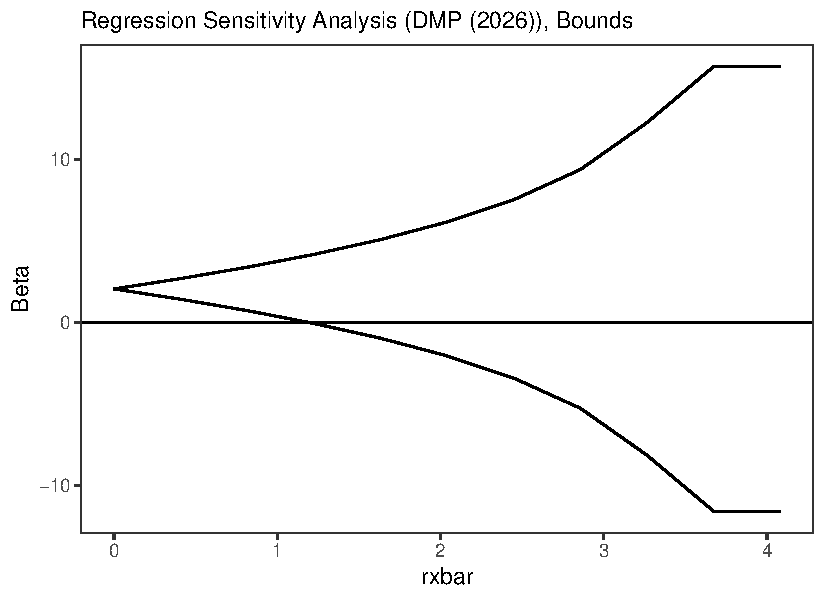
\includegraphics[width=0.85\textwidth]{figures/api-bounds-plot-1} 

}

\caption[Estimated identified set for the long-regression coefficient as a function of rxbar, holding cbar at 0.1]{Estimated identified set for the long-regression coefficient as a function of rxbar, holding cbar at 0.1. The two curves are the lower and upper bounds of the identified set; the band between them widens continuously from the point beta-med at rxbar = 0 and diverges at the finiteness threshold. The horizontal line marks the hypothesis value zero, and the breakdown point is where the lower bound crosses it.}\label{fig:api-bounds-plot}
\end{figure}
\end{Schunk}

Because the return value is a \pkg{ggplot2} object, the usual grammar
applies: adding a theme, new labels, a facet or a scale all work without
special support from the package.

\subsection{Breakdown points across control endogeneity}\label{sec:api-breakdown}

\code{regsen\_breakdown()} computes the breakdown point rather than the
whole identified set, and accepts a vector for the parameter to trace.
Sweeping \code{cbar} shows how much the robustness verdict depends on the
exogenous-controls assumption, which is the central question DMP pose.

\begin{Schunk}
\begin{Sinput}
R> bd <- regsen_breakdown(form, bfg2020, compare = w1,
+                         cbar = seq(0, 1, 0.05))
R> head(bd$results, 4)
\end{Sinput}
\begin{Soutput}
  index breakdown
1  0.00     1.350
2  0.05     1.266
3  0.10     1.195
4  0.15     1.133
\end{Soutput}
\end{Schunk}

\begin{Schunk}
\begin{Sinput}
R> plot(bd)
\end{Sinput}
\begin{figure}

{\centering 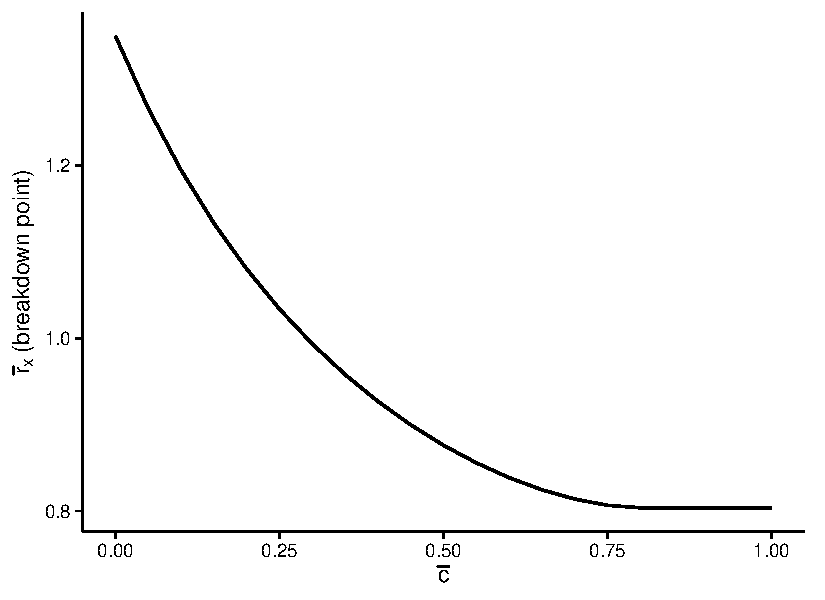
\includegraphics[width=0.85\textwidth]{figures/api-breakdown-plot-1} 

}

\caption[Estimated breakdown point for the hypothesis beta-long > 0 as a function of the bound cbar on control endogeneity]{Estimated breakdown point for the hypothesis beta-long > 0 as a function of the bound cbar on control endogeneity. Moving right relaxes the exogenous-controls assumption. The curve is monotonically decreasing and crosses one, so the robustness verdict depends materially on how endogenous the controls are assumed to be.}\label{fig:api-breakdown-plot}
\end{figure}
\end{Schunk}

Figure~\ref{fig:api-breakdown-plot} makes the paper's motivating point
concrete. Under exogenous controls the conclusion survives selection on
unobservables up to $135.0$\% of selection on observables;
under arbitrarily endogenous controls only up to
$80.4$\%. A researcher who reported only the former would
overstate robustness by a factor of about
$1.7$.

\subsection{Hypotheses other than a sign change}

By default the package tests the sign of $\bmed$ against zero. The
\code{beta} argument, together with the helpers \code{bnd\_lb()},
\code{bnd\_ub()} and \code{bnd\_eq()}, specifies other hypotheses:
\code{bnd\_lb(1)} for $\blong > 1$, \code{bnd\_eq(0)} for a two-sided
statement. Passing a vector traces the breakdown point as a function of the
hypothesized value.

\begin{Schunk}
\begin{Sinput}
R> regsen_breakdown(form, bfg2020, compare = w1, cbar = 1,
+                   beta = bnd_lb(c(0, 0.5, 1, 1.5)))$results
\end{Sinput}
\begin{Soutput}
  index breakdown
1   0.0    0.8036
2   0.5    0.7175
3   1.0    0.5753
4   1.5    0.3481
\end{Soutput}
\end{Schunk}

The breakdown point falls as the hypothesis becomes more demanding, which
it must: concluding $\blong > 1.5$ tolerates less bias than concluding
$\blong > 0$.

\subsection{The Oster (2019) analysis}\label{sec:api-oster}

Switching analyses requires only the \code{analysis} argument. Oster's
rule-of-thumb auxiliary parameter is
$R^2_{\mathrm{long}} = 1.3 R^2_{\mathrm{med}}$, obtained with
\code{r2long\_type = "relative"}.

\begin{Schunk}
\begin{Sinput}
R> o <- regsen_breakdown(form, bfg2020, compare = w1,
+                        analysis = "oster",
+                        r2long = 1.3, r2long_type = "relative",
+                        beta = bnd_eq(0))
R> o$results$breakdown
\end{Sinput}
\begin{Soutput}
[1] -23.29
\end{Soutput}
\end{Schunk}

This is the corrected Oster delta for this specification. DMP report
$-23.3$ where \citet{BFG2020} published $-8.55$; the discrepancy is the
miscomputation described in Section~\ref{sec:related}. Note that the
package returns the signed value and that $|\delta|$ is the quantity
conventionally compared to one.

\subsection{Bounding the bias magnitude directly}\label{sec:api-maxovb}

The \code{maxovb} argument implements the \citet{Masten2026} extension
described in Section~\ref{sec:related}: an explicit ceiling on
$|\bmed - \blong|$, expressed either in the units of the outcome
(\code{maxovb\_type = "bound"}) or as a fraction of $|\bmed|$
(\code{maxovb\_type = "relative"}). It is useful when a researcher can
defend a statement about how far the coefficient could move without
being willing to commit to a selection ratio.

Oster's equality analysis returns the roots of a cubic, so the identified
set can have up to three elements at each $\delta$. Adding a bias ceiling
discards the roots that violate it.

\begin{Schunk}
\begin{Sinput}
R> regsen_bounds(form, bfg2020, compare = w1, analysis = "oster",
+                delta = c(0.5, 1, 2), r2long = 1.3,
+                r2long_type = "relative",
+                maxovb = 0.5, maxovb_type = "relative")$results
\end{Sinput}
\begin{Soutput}
  delta r2long beta1 beta2 beta3
1   0.5 0.1367 2.084    NA    NA
2   1.0 0.1367 2.113    NA    NA
3   2.0 0.1367 2.173    NA    NA
\end{Soutput}
\end{Schunk}

Here the constraint is that the omitted variable cannot move the estimate
by more than half of $|\hat\bmed|$. Root columns that are \code{NA} have
been excluded by that constraint rather than failing to exist.

\subsection{The default summary}\label{sec:api-summary}

\code{regsen\_summary()} reproduces the sweep that the \Stata\ command
performs when no sub-command is given: a DMP bounds analysis at the
default grid together with an Oster breakdown analysis over a range of
$R^2_{\mathrm{long}}$ values from the rule-of-thumb value up to one. It
returns a list of two \code{regsensitivity} objects and is the quickest
way to see both analyses at once.

\begin{Schunk}
\begin{Sinput}
R> smry <- regsen_summary(form, bfg2020, compare = w1)
R> names(smry)
\end{Sinput}
\begin{Soutput}
[1] "dmp_bounds"      "oster_breakdown"
\end{Soutput}
\begin{Sinput}
R> head(smry$oster_breakdown$results, 4)
\end{Sinput}
\begin{Soutput}
   index breakdown
1 0.1367    0.9739
2 0.2367    0.9732
3 0.3367    0.9723
4 0.4367    0.9714
\end{Soutput}
\end{Schunk}

The Oster breakdown is nearly flat in $R^2_{\mathrm{long}}$ for this
specification, which is worth checking in any application: when it is
steep, the reported $\delta$ depends heavily on an auxiliary parameter
that is rarely defended.

\subsection{Calibration helpers}\label{sec:api-calib}

The reference values of Section~\ref{sec:calib} are computed by two
functions. \code{calibrate\_rho()} returns the $\rho_k$ of
\eqref{eq:rhok}, on a percentage scale, sorted by importance.

\begin{Schunk}
\begin{Sinput}
R> rho <- calibrate_rho(form, bfg2020, compare = w1)
R> rho
\end{Sinput}
\begin{Soutput}
        variable    rho
10       ave_gyi 118.34
7          d_coa  78.58
3            lon  49.93
4      temp_mean  37.26
5      rain_mean  29.29
2            lat  26.93
8          d_riv  24.96
1  log_area_2010  22.46
6      elev_mean  20.25
9          d_lak  12.06
\end{Soutput}
\end{Schunk}

These are the values of DMP Table 4 column (5), which we verify to
published precision in Section~\ref{sec:replication}. Their interpretation
is the point of the exercise: the breakdown point at $\cbar = 1$ is
$80.4$\%, which exceeds
$9$ of the
$10$ calibration values. Only \code{ave_gyi} is more
important for treatment selection than the unobservable would have to
be. If one regards the $\rho_k$ as plausible magnitudes for $r_X$, the
finding is fairly robust.

\code{calibrate\_partial\_r2()} returns $c_k^2$ from \eqref{eq:ck}, the
diagnostic for whether exogenous controls is tenable at all.

\begin{Schunk}
\begin{Sinput}
R> calibrate_partial_r2(form, bfg2020, compare = w1)
\end{Sinput}
\begin{Soutput}
        variable      R2
4      temp_mean 0.89382
2            lat 0.87613
6      elev_mean 0.68090
10       ave_gyi 0.64751
5      rain_mean 0.55878
7          d_coa 0.48721
3            lon 0.43437
8          d_riv 0.13463
9          d_lak 0.09986
1  log_area_2010 0.09813
\end{Soutput}
\end{Schunk}

Several of these are large. Under exogenous controls, $W_2$ would have a
value of zero in this table. Since the omitted variables of concern in this
application are themselves geographic and climatic, expecting
$R_{W_2 \sim W_1 \cdot W_0}$ to be near zero while the observed covariates
reach $0.89$ is difficult to defend---which is precisely why the
$\cbar$-indexed analysis is needed here.

\subsection{Bootstrap inference}\label{sec:api-boot}

The breakdown point is a statistic, and \code{regsen\_boot()} attaches a
percentile confidence interval to it. Because the \citet{BFG2020} design is
spatial, we resample whole grid cells rather than counties.

\begin{Schunk}
\begin{Sinput}
R> set.seed(2026)
R> boot <- regsen_boot(form, bfg2020,
+                      compare = w1, cbar = 1,
+                      cluster = "km_grid_cel_code",
+                      R = 199, show_progress = FALSE)
R> print(boot)
\end{Sinput}
\begin{Soutput}
Bootstrap confidence interval for the breakdown point
------------------------------------------------------------
  R                  : 199
  Cluster bootstrap  : km_grid_cel_code
  Confidence level   : 95%
  Point estimate     : 0.8036
  95% CI            : [0.5039, 0.8568]
\end{Soutput}
\end{Schunk}

The point estimate is the value DMP report as $80.4$\%. The interval is
informative for the substantive question: its lower endpoint,
$0.504$, still exceeds all but two of the $\rho_k$
values above, so the qualitative conclusion does not rest on the point
estimate alone. Omitting \code{cluster} gives the i.i.d.\ bootstrap, which
is faster but understates uncertainty when the data are spatially
correlated.

\subsection{Tracing a breakdown frontier}\label{sec:api-frontier}

The frontier \eqref{eq:bf} trades $\rxbar$ against $\rybar$. The package
does not expose it as a single call, but it is a short loop over
\code{regsen\_breakdown()}, and building it this way illustrates how the
primitives compose. For each value of $\rybar$ we ask for the $\rxbar$
breakdown point, at three levels of control endogeneity.

\begin{Schunk}
\begin{Sinput}
R> ry_grid <- c(0.5, 0.75, 1, 1.25, 1.5, 2, 3, Inf)
R> frontier <- do.call(rbind, lapply(c(0, 0.5, 1), function(cb) {
+      rx <- vapply(ry_grid, function(ry) {
+          out <- try(regsen_breakdown(form, bfg2020, compare = w1,
+                                      cbar = cb, rybar = ry),
+                     silent = TRUE)
+          if (inherits(out, "try-error")) NA_real_
+          else out$results$breakdown[1]
+      }, numeric(1))
+      data.frame(cbar = cb, rybar = ry_grid, rxbar_bp = rx)
+  }))
R> subset(frontier, cbar == 1)
\end{Sinput}
\begin{Soutput}
   cbar rybar rxbar_bp
17    1  0.50   0.9894
18    1  0.75   0.9894
19    1  1.00   0.8917
20    1  1.25   0.8039
21    1  1.50   0.8036
22    1  2.00   0.8036
23    1  3.00   0.8036
24    1   Inf   0.8036
\end{Soutput}
\end{Schunk}

\begin{Schunk}
\begin{figure}

{\centering 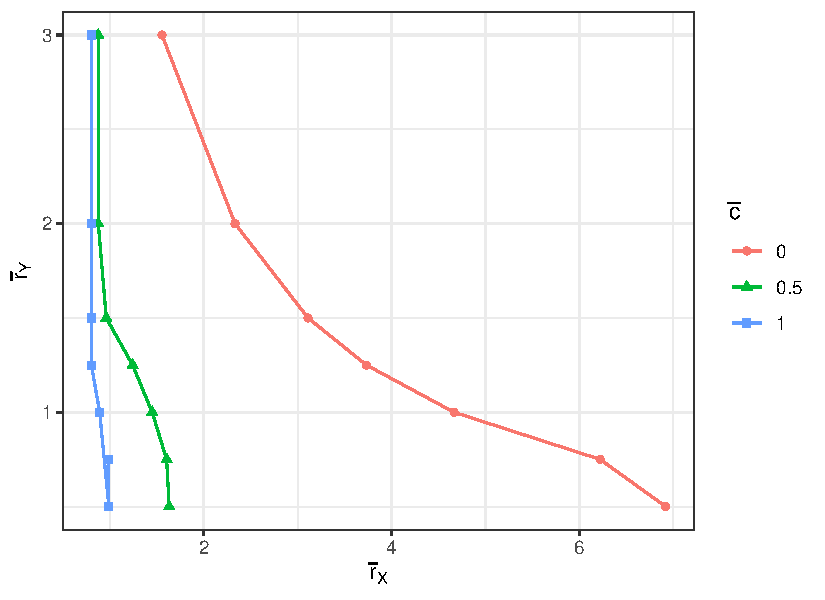
\includegraphics[width=0.85\textwidth]{figures/api-frontier-plot-1} 

}

\caption[Estimated breakdown frontiers for the hypothesis beta-long > 0]{Estimated breakdown frontiers for the hypothesis beta-long > 0. Each curve fixes a bound cbar on control endogeneity and traces the largest rxbar consistent with the conclusion, as a function of rybar. Pairs below and left of a curve are robust. Tightening cbar shifts the frontier outward, so assumptions about control endogeneity and about selection strength are substitutes.}\label{fig:api-frontier-plot}
\end{figure}
\end{Schunk}

Two things are visible. The frontier moves outward as $\cbar$ falls,
quantifying the substitution between the two assumptions noted after
\eqref{eq:thm3}. And the $\cbar = 1$ curve is confined to
$\rxbar < 0.99$, the finiteness
threshold at that $\cbar$; requesting points beyond it enters the region
Section~\ref{sec:regimes} described as uncharacterized, which is why the
loop above guards each call with \code{try()}. Users tracing frontiers at
high $\cbar$ should expect this and not mistake it for a convergence
failure.

%% ============================================================================
\section{Replicating Diegert, Masten and Poirier (2026)}\label{sec:replication}
%% ============================================================================

The package ships a test suite that pins its output to the published values
of the paper it implements. This section reports the comparison; the
assertions themselves live in
\code{tests/testthat/test-paper-table1.R} and run on every check.



Table~\ref{tab:replication} collects the results. All twenty-six assertions
pass. Four values differ from the published figure in the last printed
digit, which we report explicitly rather than rounding away. Three are in
DMP Tables 3 and 4: our $\hat c_k^2$ for average temperature is $0.8938$
against a published $0.893$, for average rainfall $0.5588$ against
$0.560$, and our $\hat\rho_k$ for elevation is $20.25$ against $20.2$. The
fourth is in Table~\ref{tab:replication} itself, where our
$\hat{\overline{r}}^{\mathrm{bp}}$ of $95.8$\% is printed
as $95.9$\% by DMP. Every entry agrees to within $0.07$, and the pattern
is consistent with rounding in the published tables rather than with a
difference in estimand. We flag them because a reader checking the
implementation against the paper would otherwise wonder.

\begin{table}[t!]
\centering
\begin{tabular}{llll}
  \toprule
Quantity & Published & Package & Source \\ 
  \midrule
$\hat\beta_{\mathrm{med}}$ & 2.055 & 2.055 & Table 1, Panel A \\ 
  Number of counties & 2,036 & 2,036 & Table 1, Panel A \\ 
  Mean of dependent variable & 60.04 & 60.04 & Table 1, Panel A \\ 
  $\hat\delta^{\mathrm{bp}}_{\mathrm{resid}}$ (corrected) & -23.3 & -23.3 & Table 1, Panel B \\ 
  $\hat{\overline{r}}^{\mathrm{bp}}_X$ (\%) & 80.4 & 80.4 & Table 1, Panel C \\ 
  $\hat{\overline{r}}^{\mathrm{bp}}$ (\%) & 95.9 & 95.8 & Table 1, Panel C \\ 
   \bottomrule
\end{tabular}
\caption{Replication of \citet{Diegert2026} Table 1, column (5).
    Published values are as printed in that paper; package values are
    computed by the code in this section. Tables 3 and 4 of that paper are
    replicated entry by entry in Sections~\ref{sec:api-calib}
    and~\ref{sec:replication}.} 
\label{tab:replication}
\end{table}


Two of these deserve comment. The corrected Oster delta of
$-23.3$ reproduces DMP's correction of the published
$-8.55$, which is a useful check that the package implements Proposition 3
of \citet{Oster2019} rather than the shortcut that produced the original
number. And the ordering
$\hat{\overline{r}}^{\mathrm{bp}}_X = 80.4\%
\le \hat{\overline{r}}^{\mathrm{bp}} = 95.8\%$
is the inequality guaranteed at the end of Section~\ref{sec:rybar},
obtained here through two entirely different code paths---the closed form
\eqref{eq:cor1} and a bisection over DIRECT-L solves---which makes it a
genuine consistency check rather than a tautology.

%% ============================================================================
\section{Application: California test scores}\label{sec:case-school}
%% ============================================================================

The \citet{StockWatson2011} treatment of the \code{CASchools} data,
distributed with \pkg{AER} \citep{AER}, is a canonical applied regression
and a useful second illustration because the substantive question---whether
smaller classes raise test scores---has an obvious omitted-variable
concern. We regress the average of reading and mathematics scores on the
student--teacher ratio, using the English-learner share and the
free-lunch share as calibration covariates and county fixed effects as
controls.

\begin{Schunk}
\begin{Sinput}
R> suppressPackageStartupMessages(library("AER"))
R> data("CASchools", package = "AER")
R> CASchools$score <- with(CASchools, (read + math) / 2)
R> CASchools$STR   <- CASchools$students / CASchools$teachers
R> 
R> f <- score ~ STR + english + lunch + county
R> res <- regsen_bounds(f, CASchools, compare = c("english", "lunch"),
+                       cbar = 1)
R> res$dgp$beta_med
\end{Sinput}
\begin{Soutput}
[1] -0.9011
\end{Soutput}
\begin{Sinput}
R> res$breakdown
\end{Sinput}
\begin{Soutput}
[1] 0.9446
\end{Soutput}
\end{Schunk}



The medium regression gives
$\hat\bmed = -0.901$: a one-unit increase in the
student--teacher ratio is associated with a
$0.90$-point lower average score. The
breakdown point at $\cbar = 1$ is
$0.945$, so the negative-effect conclusion survives
unless selection on unobservables is at least
$94.5$\% as strong as selection on the two
calibration covariates. Under exogenous controls the figure is
$2.878$.

This is a case where calibration changes the reading. The two $\rho_k$
values are $115.9$\% and
$86.3$\%, so the breakdown point at $\cbar = 1$
lies below the larger of them. An unobservable no more important for
class-size selection than the free-lunch share is already enough to
overturn the sign.
The bootstrap interval, $[0.531,
0.997]$ over $R = 199$ i.i.d.\ replicates, does
not change that assessment. Compared with the frontier application of
Section~\ref{sec:api}---where the breakdown point exceeded nine of ten
calibration values---this specification is considerably less robust, and
the contrast illustrates why a breakdown point should never be read against
a universal cutoff.

%% ============================================================================
\section{Simulation: coverage of the bootstrap interval}\label{sec:case-sim}
%% ============================================================================

Bootstrap inference on the breakdown point is the package's main addition
to the methodology, so it needs evidence rather than assertion. This
section reports a simulation study of its finite-sample coverage. We use a
design in which the omitted variable is correlated with a calibration
covariate, so that control endogeneity is present by construction:
\begin{align*}
W_{1a}, W_{1b} &\sim N(0, 1), \qquad
W_2 = \rho W_{1a} + \sqrt{1 - \rho^2}\, \varepsilon, \\
X &= 0.5 W_{1a} + 0.3 W_{1b} + 0.5 W_2 + \nu, \\
Y &= 1.0 X + 0.3 W_{1a} + 0.2 W_{1b} + 0.4 W_2 + u,
\end{align*}
with $\rho = 0.5$ and all disturbances standard normal. Because the
breakdown point is a functional of the population variance matrix rather
than a structural parameter, there is no closed-form ``true'' value to
compare against; we therefore compute a pseudo-true value on a single
sample of $4 \times 10^5$ observations and treat that as the target. For
each sample size we draw $M$ independent samples, compute a percentile
interval from $R$ bootstrap replicates, and record whether it covers.





\begin{table}[t!]
\centering
\begin{tabular}{rrrrr}
  \toprule
$n$ & Coverage (\%) & Bias & SD & Mean CI width \\ 
  \midrule
500 & 92.0 & -0.0053 & 0.0294 & 0.1122 \\ 
  1000 & 92.0 & -0.0030 & 0.0208 & 0.0799 \\ 
  4000 & 95.6 & 0.0001 & 0.0097 & 0.0395 \\ 
   \bottomrule
\end{tabular}
\caption{Finite-sample performance of the percentile bootstrap interval for the breakdown point, at nominal 95\% level. $M = 250$ Monte Carlo replications, $R = 199$ bootstrap draws each, $\bar c = 1$. The pseudo-true breakdown point is 0.7170, computed on a single sample of $4 \times 10^5$ observations. Bias and SD refer to the point estimator of the breakdown point.} 
\label{tab:coverage}
\end{table}


Table~\ref{tab:coverage} supports a qualified endorsement. The point
estimator is close to unbiased at every sample size and its dispersion
falls at the expected rate. Coverage improves with $n$ and is close to
nominal by $n = 4000$, but at $n = 500$ the interval under-covers, at
$92.0$\% against a nominal $95$\%. The
direction is what one would expect: the breakdown point is a smooth but
nonlinear functional of an estimated variance matrix, and the percentile
interval inherits the resulting finite-sample skewness without correcting
for it.

The practical recommendation is therefore to treat the interval as
approximate in small samples, and to prefer the cluster bootstrap whenever
the design has a grouping structure, as in Section~\ref{sec:api-boot}.
Bias-corrected or accelerated intervals are a natural improvement and are
not currently implemented; we note this as the most useful direction for
future work on the package.

%% ============================================================================
\section{Comparison with sensemakr}\label{sec:compare}
%% ============================================================================

\pkg{sensemakr} \citep{sensemakr} implements \citet{Cinelli2020} and is the
tool an \Rlang\ user is most likely to reach for. As
Table~\ref{tab:crosswalk} indicated, the two packages parameterize the same
bias decomposition \eqref{eq:chbias} differently, and it is worth seeing
the numbers side by side on one specification.

\begin{Schunk}
\begin{Sinput}
R> suppressPackageStartupMessages(library("sensemakr"))
R> fit <- lm(form, data = bfg2020)
R> sm <- sensemakr(model = fit, treatment = "tye_tfe890_500kNI_100_l6",
+                  benchmark_covariates = w1, kd = 1, ky = 1,
+                  q = 1, alpha = 0.05, reduce = TRUE)
R> sm$sensitivity_stats[c("r2yd.x", "rv_q", "rv_qa")]
\end{Sinput}
\begin{Soutput}
   r2yd.x   rv_q  rv_qa
1 0.03931 0.1829 0.1463
\end{Soutput}
\end{Schunk}



The robustness value is $RV_{q=1} = 0.1829$: an unobservable
explaining more than $18.3$\% of the residual variation in
\emph{both} treatment and outcome would suffice to bring the estimate to
zero. The partial $R^2$ of treatment with outcome is
$0.0393$. \pkg{regsensitivity} reports, for the same
specification, a breakdown point of $80.4$\% at
$\cbar = 1$.

These two numbers are not comparable, and the temptation to compare them is
the main hazard in using both packages. $RV_q$ is a partial $R^2$, bounded
by one by construction and measured against the residual variation in the
data. The breakdown point is a ratio of index standard deviations, measured
against the explanatory power of the chosen calibration covariates. A
specification with weak controls will have a high breakdown point and an
unchanged $RV_q$. The right way to read them jointly is as answers to
different questions: $RV_q$ asks how strong an unobservable must be in
absolute explanatory terms, and $\rxbar^{\mathrm{bp}}$ asks how strong it
must be relative to what we have already adjusted for.

The substantive difference is the treatment of the controls. Because
\pkg{sensemakr} conditions on exogenous controls, its benchmark bounds
are computed by asking how large an unobservable ``$k$ times as strong as''
a named covariate would be, holding the control structure fixed. As
Section~\ref{sec:api-calib} showed, the calibration covariates in this
application have partial $R^2$ against one another as high as $0.89$, so
the premise is doubtful and a $\cbar$-indexed analysis is the more
defensible one. Where the controls are genuinely exogenous the two
approaches are complementary, and we recommend reporting both. A
reproducible version of this comparison is bundled at
\code{inst/benchmarks/sensemakr-comparison.R}.

%% ============================================================================
\section{Performance}\label{sec:bench}
%% ============================================================================

Table~\ref{tab:timing} reports median single-call timings on the
\citet{BFG2020} application ($n = 2036$, ten calibration controls plus
state fixed effects). The pattern follows the regime dispatch of
Section~\ref{sec:regimes}: everything in a closed-form regime costs a few
milliseconds, and the DIRECT-L regime costs about a second. The bundled
script \code{inst/benchmarks/performance.R} regenerates every row.

\begin{table}[t!]
\centering
\begin{tabular}{lr}
\toprule
Call & Median (ms) \\
\midrule
DMP bounds, $\rybar = \infty$, $\cbar = 0.1$, 10 grid points & 6.1 \\
DMP bounds, $\rybar = 2$, $\cbar = 1$, 10 grid points (DIRECT-L) & 993 \\
DMP breakdown across $\cbar$, 11 grid points & 5.6 \\
Oster bounds (equality), 21 $\delta$ values & 6.9 \\
Oster breakdown (sign hypothesis) & 5.6 \\
Cluster bootstrap, $R=99$, BFG application & 1{,}038 \\
Bootstrap (no clustering), $R=99$, BFG application & 595 \\
\bottomrule
\end{tabular}
\caption{Median timings over five runs on an Apple M4 laptop under
\proglang{R}~4.5.2. The DIRECT-L regime is roughly two orders of magnitude
slower because it solves a nonconvex global optimization at every grid
point; see Section~\ref{sec:regimes}.}
\label{tab:timing}
\end{table}

For context, DMP report that the breakdown-frontier computation for their
application takes ``about 15 seconds on a standard machine.'' The
corresponding \pkg{regsensitivity} call is the third row of
Table~\ref{tab:timing}. The gain comes from the staging described in
Section~\ref{sec:software}: the variance summary is computed once and
reused across every point on the grid, rather than recomputed per
evaluation.

%% ============================================================================
\section{Summary and discussion}\label{sec:concl}
%% ============================================================================

\pkg{regsensitivity} brings the \citet{Diegert2026}, \citet{Oster2019} and
\citet{Masten2026} analyses into \Rlang\ as a single coherent package. Its
distinguishing feature relative to the existing ecosystem surveyed in
Section~\ref{sec:landscape} is that it does not require the included
controls to be exogenous, and that it treats the breakdown point as a
first-class object which can be traced against a second sensitivity
parameter, plotted, and bootstrapped. Section~\ref{sec:replication}
verifies the implementation against every published value of
\citet{Diegert2026} Table 1 column (5) and Tables 3 and 4, pinned by 26
regression tests so that future changes announce themselves.

Three limitations are worth stating plainly. First, the package implements
Assumption A6 only in the one-sided form $[0, \cbar]$; DMP's general
two-sided restriction $[\clow, \cbar]$, which is useful when a researcher
wants to assert that controls are \emph{at least} somewhat endogenous, is
not available. Second, the region
$\rxbar > r_{\max}(\cbar) > \rybar$ is uncharacterized in the underlying
theory and the package raises an error there rather than guessing;
Section~\ref{sec:api-frontier} shows when a user meets this boundary.
Third, the bootstrap interval is a percentile interval and, as
Section~\ref{sec:case-sim} documents, under-covers at $n = 500$. Adding
bias-corrected and accelerated intervals is the highest-value extension we
can identify, and the simulation harness in Section~\ref{sec:case-sim}
provides the yardstick against which to judge it.

The package, with its five vignettes---a tour, a paper-replication
walk-through, a stylized illustration of the Masten--Poirier
extensions, a plotting-and-tables guide, and a Stata migration
guide---is available at
\url{https://github.com/mikenguyen13/regsensitivity}.

%% ============================================================================
\section*{Computational details}
%% ============================================================================

The results in this paper were obtained using
\proglang{R}~4.5.2
on aarch64-apple-darwin20, with the packages
\pkg{regsensitivity}~0.1.2,
\pkg{ggplot2}~4.0.0,
\pkg{nloptr}~2.2.1,
\pkg{AER}~1.2.15,
\pkg{sensemakr}~0.1.6 and
\pkg{knitr}~1.50.
\proglang{R} itself and all packages used are available from the
Comprehensive \proglang{R} Archive Network (CRAN) at
\url{https://CRAN.R-project.org/}. Every number, table and figure in this
paper is regenerated by the replication script \code{paper.R} distributed
with the manuscript; the two computationally expensive
chunks---the breakdown frontier of Section~\ref{sec:api-frontier} and the
coverage study of Section~\ref{sec:case-sim}---are cached, and the full
build takes a few minutes from a cold cache.

%% ============================================================================
\section*{Acknowledgments}
%% ============================================================================

This \Rlang\ package implements the methodology of \citet{Diegert2026},
\citet{Oster2019} and \citet{Masten2026}. The package internals follow the
structure of the \Stata\ code released by Diegert, Masten and Poirier
alongside their paper, and several internal function names are retained
from it to make the two implementations comparable.

\bibliography{paper}

\newpage
\begin{appendix}

%% ============================================================================
\section{From the identified set to the breakdown point}\label{app:deriv}
%% ============================================================================

The closed form for the breakdown point in \eqref{eq:cor1} follows from
Theorem 1 by a short argument that is worth setting out, because it makes
clear why $\rxbar^{\mathrm{bp}} < 1$ is a property of the
arbitrarily-endogenous-control case rather than a general fact.

Take $\bmed > 0$ and the hypothesis $\blong > 0$. By \eqref{eq:thm1} the
identified set is the interval $\bmed \pm \mathrm{dev}(\rxbar)$, so the
hypothesis holds for every element of the set exactly when
$\bmed - \mathrm{dev}(\rxbar) \ge 0$. Since $\mathrm{dev}$ is continuous
and strictly increasing in $\rxbar$ on the region where the bounds are
finite, and $\mathrm{dev}(0) = 0$, the supremum in \eqref{eq:bpdef} is
attained where the lower bound just touches zero:
\begin{equation}
\mathrm{dev}(\rxbar^{\mathrm{bp}}) = \bmed .
\label{eq:appdev}
\end{equation}
Substituting \eqref{eq:dev} and writing $\lambda := \Rsq{X \sim W_1}$ and
$V := \Var(Y^{\perp X, W_1}) / \Var(X^{\perp W_1})$, condition
\eqref{eq:appdev} is
\[
\frac{\rxbar^2 \lambda}{1 - \lambda - \rxbar^2 \lambda} \cdot V
= \bmed^2 .
\]
Solving for $\rxbar^2$ gives
\[
\rxbar^2 = \frac{\bmed^2 (1 - \lambda)}
                {\lambda \left(V + \bmed^2\right)},
\]
and rewriting $\bmed^2 / (V + \bmed^2)$ as the partial $R^2$ of the
outcome on treatment, $\Rsq{Y \sim X \cdot W_1}$, yields
\eqref{eq:cor1}. The ceiling is now visible: the right-hand side of
\eqref{eq:cor1} is a ratio whose denominator exceeds its numerator by
$(1 - \lambda)/\lambda > 0$, so $\rxbar^{\mathrm{bp}} < 1$ whenever
$\lambda < 1$. Under Theorem 3 the deviation function is driven by
$\overline{z}_X(\rxbar, \clow, \cbar)$ instead, and restricting $\cbar$
below one slows its growth in $\rxbar$, which is what allows the
breakdown point to exceed one---as it does at
$\cbar \in \{0, 0.1\}$ in Section~\ref{sec:api-bounds}.

The same argument run against a general hypothesis value $b$ rather than
zero replaces $\bmed$ by $|\bmed - b|$ throughout, which is why the
breakdown points reported in Section~\ref{sec:api} decline as $b$ moves
toward $\bmed$.

%% ============================================================================
\section{Reproducing the results in this paper}\label{app:repro}
%% ============================================================================

Every number, table and figure above is produced by the replication script
\code{paper.R} distributed with this manuscript, which runs top to bottom
in a clean session. Its structure follows the sections of the paper. The
two expensive steps are the breakdown frontier of
Section~\ref{sec:api-frontier} and the coverage study of
Section~\ref{sec:case-sim}; in the manuscript these are \pkg{knitr}-cached,
and in the standalone script they are plain code with their run times noted
in comments.

The regression tests that pin the replicated values are run with

\begin{Code}
R> testthat::test_local()
\end{Code}

from the package source, or on the installed package with

\begin{Code}
R> testthat::test_package("regsensitivity")
\end{Code}

The benchmark timings of Table~\ref{tab:timing} and the \pkg{sensemakr}
comparison of Section~\ref{sec:compare} are regenerated by

\begin{Code}
R> source(system.file("benchmarks", "performance.R",
+                     package = "regsensitivity"))
R> source(system.file("benchmarks", "sensemakr-comparison.R",
+                     package = "regsensitivity"))
\end{Code}

\end{appendix}

\end{document}
